%%%%%%%%%%%%%%%%%%%%%%%%%%%%%%%%%%%%%%%%%%%%%%%%%%%%%%%%%%%%%%%%%%%%
% Authors: A. Herrera-Poyatos, F. Herrera
% Tittle: Algoritmo memético equilibrado con diversificación voraz
% 							 CAEPIA 2015
%%%%%%%%%%%%%%%%%%%%%%%%%%%%%%%%%%%%%%%%%%%%%%%%%%%%%%%%%%%%%%%%%%%%

\section{Big Data}

	\subsection*{¿Qué es Big Data?}

		\begin{frame}{Definiciones}

			\begin{tcolorbox}[colback=blue!5,colframe=blue!15]
				Un problema sobre datos entra en el ámbito de Big Data cuando la aplicación de las actuales tecnologı́as no permite al usuario obtener soluciones rápidas, efectivas en costo y de calidad.
			\end{tcolorbox}
		\end{frame}

		\begin{frame}{Las 3 Vs de Big Data}
			\kern -0.5cm
			\fontsize{6}{8}\selectfont
			\begin{tikzpicture}
			\node (img1) {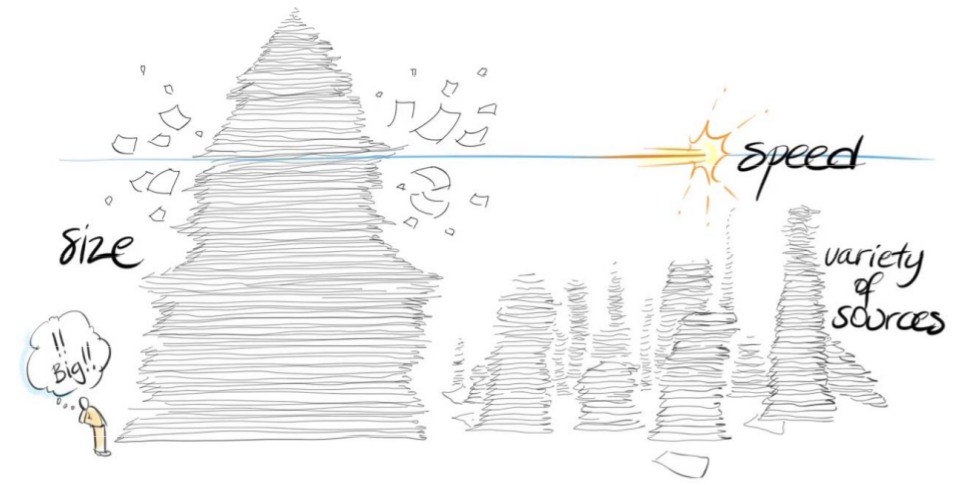
\includegraphics[width=\textwidth]{./Images/big-data-vs.png}};
			\node [fill=Grandis!80, circle,inner sep=0.5pt, text width=1.35cm, align=center, above right = 2cm and 2cm of $(img1)$] (vel) {Velocidad};
			\node [fill=TurkishRose!80, circle,inner sep=0.5pt, text width=1.35cm, align=center, right= 1.6cm of $(vel)$] (var) {Variedad};
			\node [fill=ChetwodeBlue!80, circle, inner sep=0.5pt, text width=1.35cm, align=center, above = 9mm of $(vel)!0.5!(var)$] (vol) {Volumen};
			\node [fill=Jaguar!85, circle, inner sep=0.5pt, text width=1.5cm, align=center, below = 4mm of $(vol)$] (bd) {\color{white}{\textbf{Big Data}}};
			\end{tikzpicture}

		\end{frame}

	
	\subsection*{Campos relacionados}

		\begin{frame}{Business intelligence}
			
			
		\end{frame}
		
		\begin{frame}{Ciencia de datos}
			
			
		\end{frame}
		

	\subsection*{Big Data e ingeniería de servidores}
	
		\begin{frame}{GFS}
			
			
		\end{frame}